Un \textbf{Non-Fungible Token} (\textbf{NFT}) è un tipo speciale di token che rappresenta l'atto di proprietà, nonchè il certificato di autenticità, scritto su blockchain, di un bene unico digitale o fisico. Tali token quindi non sono reciprocamente intercambiabili e per tale motivo sono in contrapposizione con le criptovalute come Bitcoin, le quali sono per stessa natura fungibili, ossia possono essere duplicati infinite volte in copie identiche e intescambiabili. Gli NFT invece si differenziano per il fatto che è possibile definirne univocamente un'identità del singolo token che lo differenzia da tutti gli altri. Tali token sono diventati virali per la prima volta quando \textbf{CryptoKitties} \cite{web:ck} è diventato virale e dai cui tale progetto ha tratto forti spunti.

Infine gli NFT sono stati una vera e propria rivoluzione nel campo del diritto d'autore dal momento che permette a chi ne acquista uno di ottenere un certificato che gli consente di tenere traccia e provare la proprietà della copia, digitale o non, acquistata.

\begin{figure}[h]
    \centering
    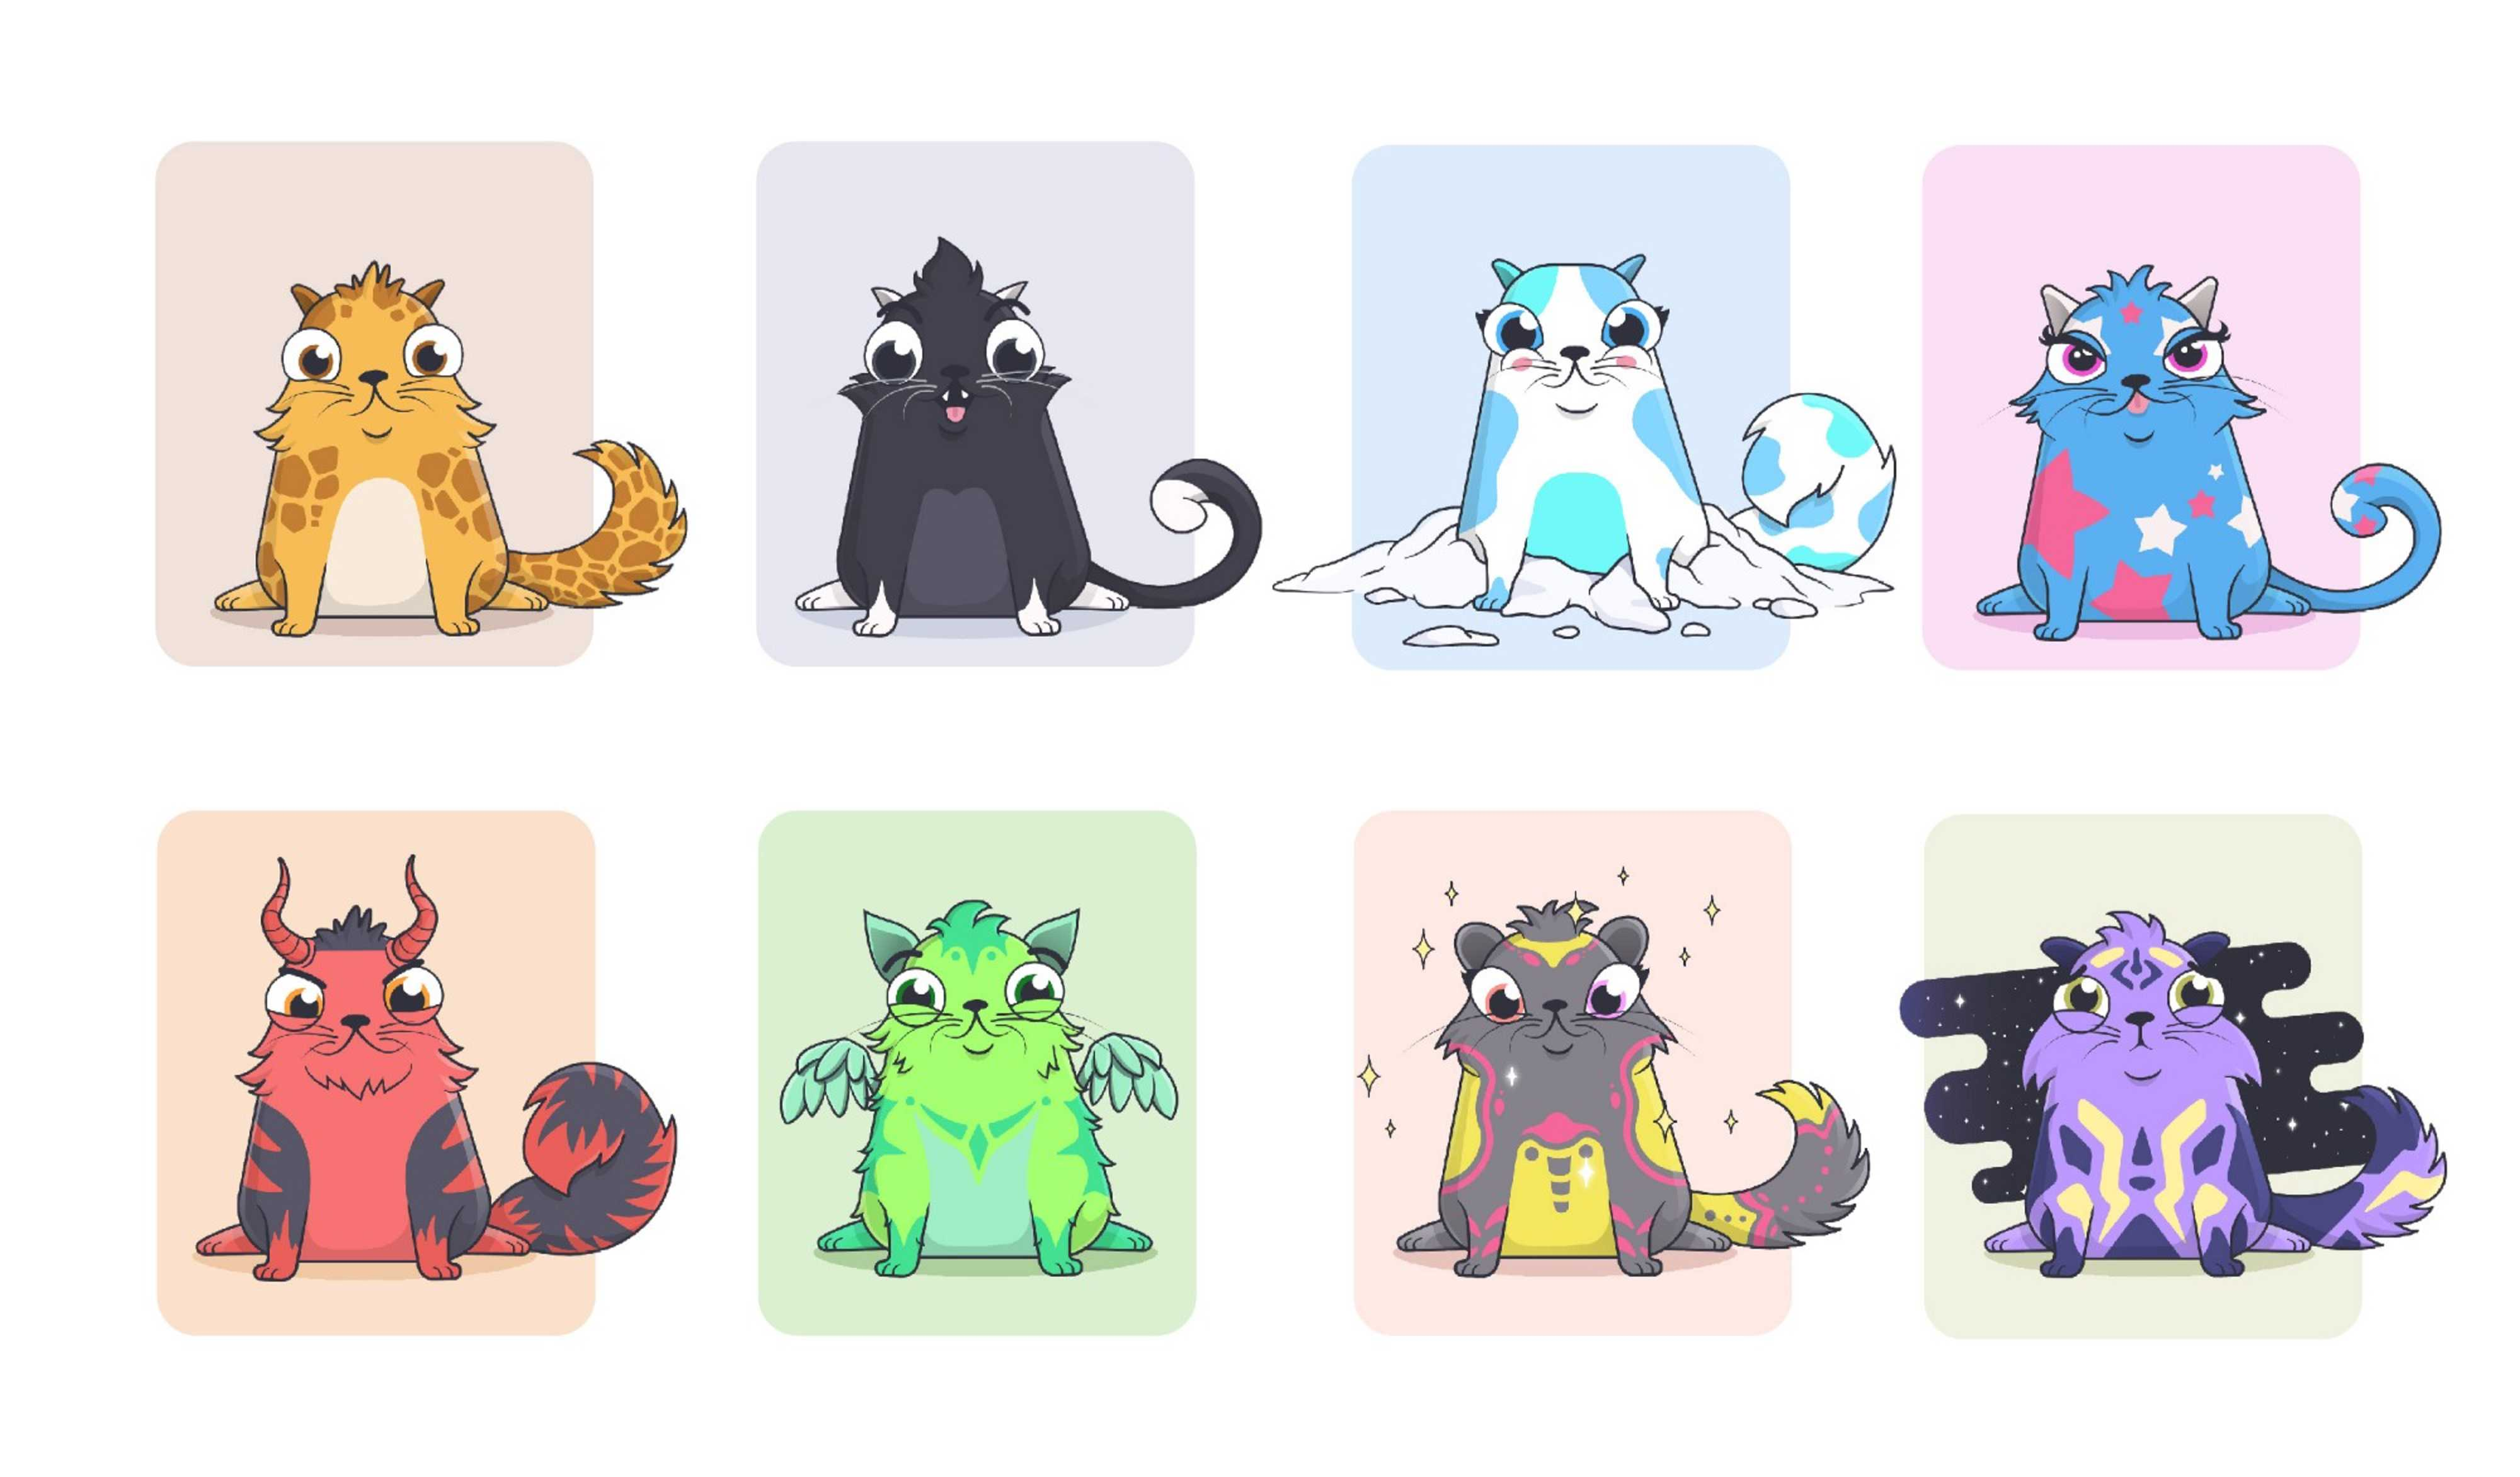
\includegraphics[width=0.68\textwidth]{tesina/img/NFT.png}
    \caption{Esempio di CryptoKitties NFT}
\end{figure}